
\section{ElasticSearch}

\subsection{Installation}

Die Installation ist bei ElasticSearch dreigeteilt. Um ElasticSearch in dem Umfang nutzen zu können, wie es hier gewünscht ist, muss zum einen ElasticSearch, Kibana als auch Logstash installiert werden. ElasticSearch ist hierbei das Kernstück und dient als Datenbank. Kibana ist eine grafische Benutzeroberfläche für ElasticSearch und Logstash stellt die Brücken zwischen der MySQL-Datenbank und ElasticSearch dar. Während ElasticSearch Java mitgeliefert hat, muss für Logstash Java Version 8 oder 11 nachinstalliert werden. Um die drei Dienste für den Development Modus zu installieren, mussten nur die Archive entpackt und die entsprechenden Anwendungen gestartet werden. Ohne die Konfigurationsdateien zu ändern, konnten die Anwendungen direkt miteinander kommunizieren. Allerdings wirf Logstash beim Start ein paar Warnungen, welche wohl mit JRuby zusammenhängen und den Entwicklern schon bekannt sind. Diese können hier ignoriert werden.

Für eine richtige Installation gibt es mehrere Wege, entweder man fügt deren Repository ein, verwendet das bereitgestellte Debian-Paket oder installiert es per Docker. Für diesen Test habe ich mich für das Debian-Paket entschieden. 

\subsection{Indexierung}

Um nun Daten zu indexieren, muss in einer Conf-Datei in Logstash definiert werden, wie und welche Daten gelesen und weitergegeben werden sollten \ref{lst:lsConf}. Dabei kann Logstash direkt MySQL-Querys gegen die Datenbank stellen. Die Datei ist in zwei Blöcke unterteilt. Zum einen ein Input-Block, welcher erklärt, welche Daten eingelesen werden sollen und einen Output Block, welcher das Ziel für die Daten angibt. Für den Input Block verwende ich hier den MariaDB-Treiber. Dabei kam es bei dem System allerdings zu Problemen. Der Treiber konnte über den in der Dokumentation angegeben Weg nicht geladen werden.  Der Treiber musste direkt im Core von Logstash mitgeladen werden, damit er funktioniert. Deswegen ist die Zeile mit dem Pfad zur Bibliothek auch leer. Nachdem die Datenbank Konfiguration und Query angegeben wurden, kann noch ein Zeitplan definiert werden. Dieser stellt ein, wie oft der Query startet werden soll. Zudem ist es auch möglich, eine Art Delta-Query zu defieren, dafür wird eine Tracking-Column festgelegt, welche dann in der Query auf einen Zeitstempel überprüft wird.
Im zweiten Teil der Datei wird das Ziel definiert. Die erste Zeile dient dazu nur dem Debugging, da es alle ausgegeben Linien des Skripts auch auf die Shell herausgibt. In dem ElasticSearch-Segment wird zum einen eine ID definiert, welche verhindert, dass Einträge doppelt in die Datenbank gespielt werden. Dewegen wird hier die ID der Lemmata genommen, da diese auch in der Datenbank nicht wiederholt werden darf. Danach gibt man noch den Index und DokumentenTyp an, welcher für die erhaltenen Daten angelegt wird. 
Als die Indexierung nun gestartet wurde, kam es allerdings zu einem Fehler. Dieser sagte aus, dass eine Zählung der erwarteten Ergebnisse, welche von Logstash abgesetzt wurde, keine gültige MySQL-Query sei. Dies lag daran, dass Logstash Double anstelle von Single-Quotes verwendete. Dies konnte behoben werden, indem eine Einstellung in der Datenbank vorgenommen wurde, um auch Double-Quotes zu erlauben. 
Danach verlief die Indexierung ohne weitere Probleme.

\begin{lstlisting}[language=json, frame=single, label={lst:lsConf}] 
  input {
    jdbc {
      jdbc_validate_connection => true
      jdbc_driver_library => ""
      jdbc_driver_class => "Java::org.mariadb.jdbc.Driver"
      jdbc_connection_string =>
          "jdbc:mariadb://localhost:3306/dietrichonline"
      jdbc_user => "USER"
      jdbc_password => "PW"
      tracking_column => "timestamp"
      use_column_value=>true
      statement => "MYSQL-Query WHERE timestamp > :sql_last_value"
      schedule => "0 */6 * * *"
    }
  }
  
  output {
    stdout { codec => json_lines }
    elasticsearch {
      document_id => "%{id}"
      document_type => "lemma"
      index => "lemma"
      hosts => "localhost:9200"
    }
  }
\end{lstlisting}

Nun ist die Frage jedoch, wie weiß ElasticSearch, was für ein Datentyp das Feld besitzt. Dafür verwendet ElasticSearch ein sogenanntes Dynamic Mapping, indem es versucht den am besten passenden Datentyp für das Feld zu finden. In diesem Text wurden die meisten Felder als Strings erkannt und so gesetzt. Dies ist für diesen Kurztest ausreichend. 

\subsection{Oberfläche}

Die Oberfläche von Kibana bietet eine zu Beginn überwältigende Erfahrung. Allerdings können Sichten für verschiedene Nutzer angelegt werden. Zudem gibt es ein Login-System, welcher allerdings erst aktiviert werden muss. Es gibt viele Menüpunkte, welche es ermöglichen die Daten auf diverse Arten darzustellen. Darunter in Graphen-Form und auf einer Landkarte. Unter dem Punkt Management finden sich die Einstellungen für das ElasticSearch System. Hier kann man nicht nur Snapshots erstellen, sondern auch das System mit Updates versorgen. Zudem können hier die Indices verwaltet werden \ref{img:elasticInterface}. Eine Erstellung ist allerdings nur per API möglich. Auch ist es möglich Indizes eine Lebensdauer zu geben. Die Oberfläche ist vollkommen responsive. Neben diesem Menü gibt es ebenfalls eine Entwicklerkonsole, in der es möglich ist Anfragen an das ElasticSearch-System zu schicken. 


\begin{figure}
	\centering
	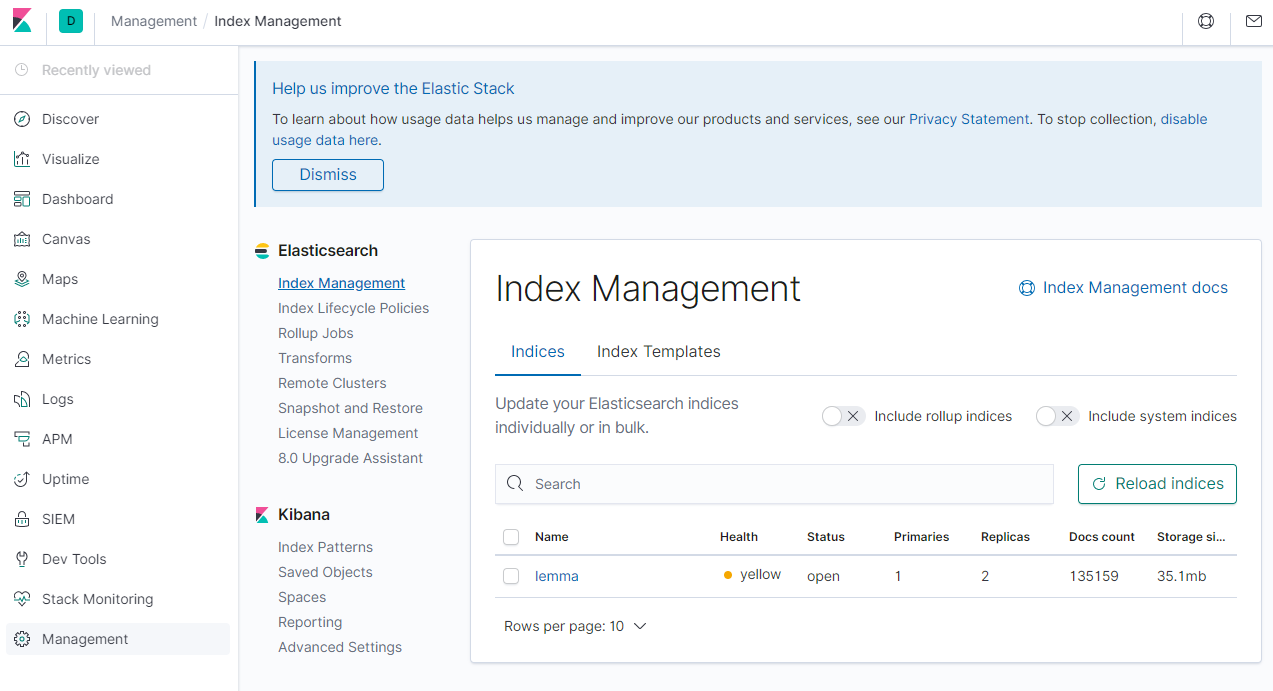
\includegraphics[width=1\linewidth]{images/elastic_ui.png}
	\caption{Index Managment Seite von ElasticSearch}
	\label{img:elasticInterface}
\end{figure}


\subsection{Dokumentation}



Bei der Informationsseite zum PHP-Klienten ist allerdings ein kleiner Fehler auf der Seite. Die benötige PHP-Version ist dort falsch vermerkt.



\subsection{Absetzen einer Anfrage und Integration in PHP}

ElasticSearch bietet einen eigenen PHP-Klienten an. Dieser kann mit Composer installiert werden.

